\subsection{Adding External Knowledge}
\label{sec:wiki}

% All of the wikipedia inclusion work.

Motivated by the intuition that phrases gain importance because of both their role in a document and their semantic meaning in the broader world, we experimented with multiple algorithms that incorporate outside knowledge. Each algorithm integrates Wikipedia as a knowledge source in different ways.

\subsubsection{Boosting Documents}

The first algorithm concatenates to each lecture a closely related Wikipedia page,
and then uses the previously described statistical and linguistic techniques
to choose phrases from the combined document. Formally, the procedure is as
follows.

For example, for the lecture titled ``View Modifications Using
Triggers'', the first page in the Wikipedia search results is
``Database trigger'', which is then concatenated to the transcript of
the lecture. Then, using either n-grams or adjective-noun phrases as
candidate keywords, the algorithm chooses phrases with TF-IDF over the
combined document for the index.

\begin{figure}
\caption{The Document Boosting algorithm searches for a Wikipedia page using the title of the lecture, concatenates the result to the lecture, and then runs TF-IDF over the combined document.}
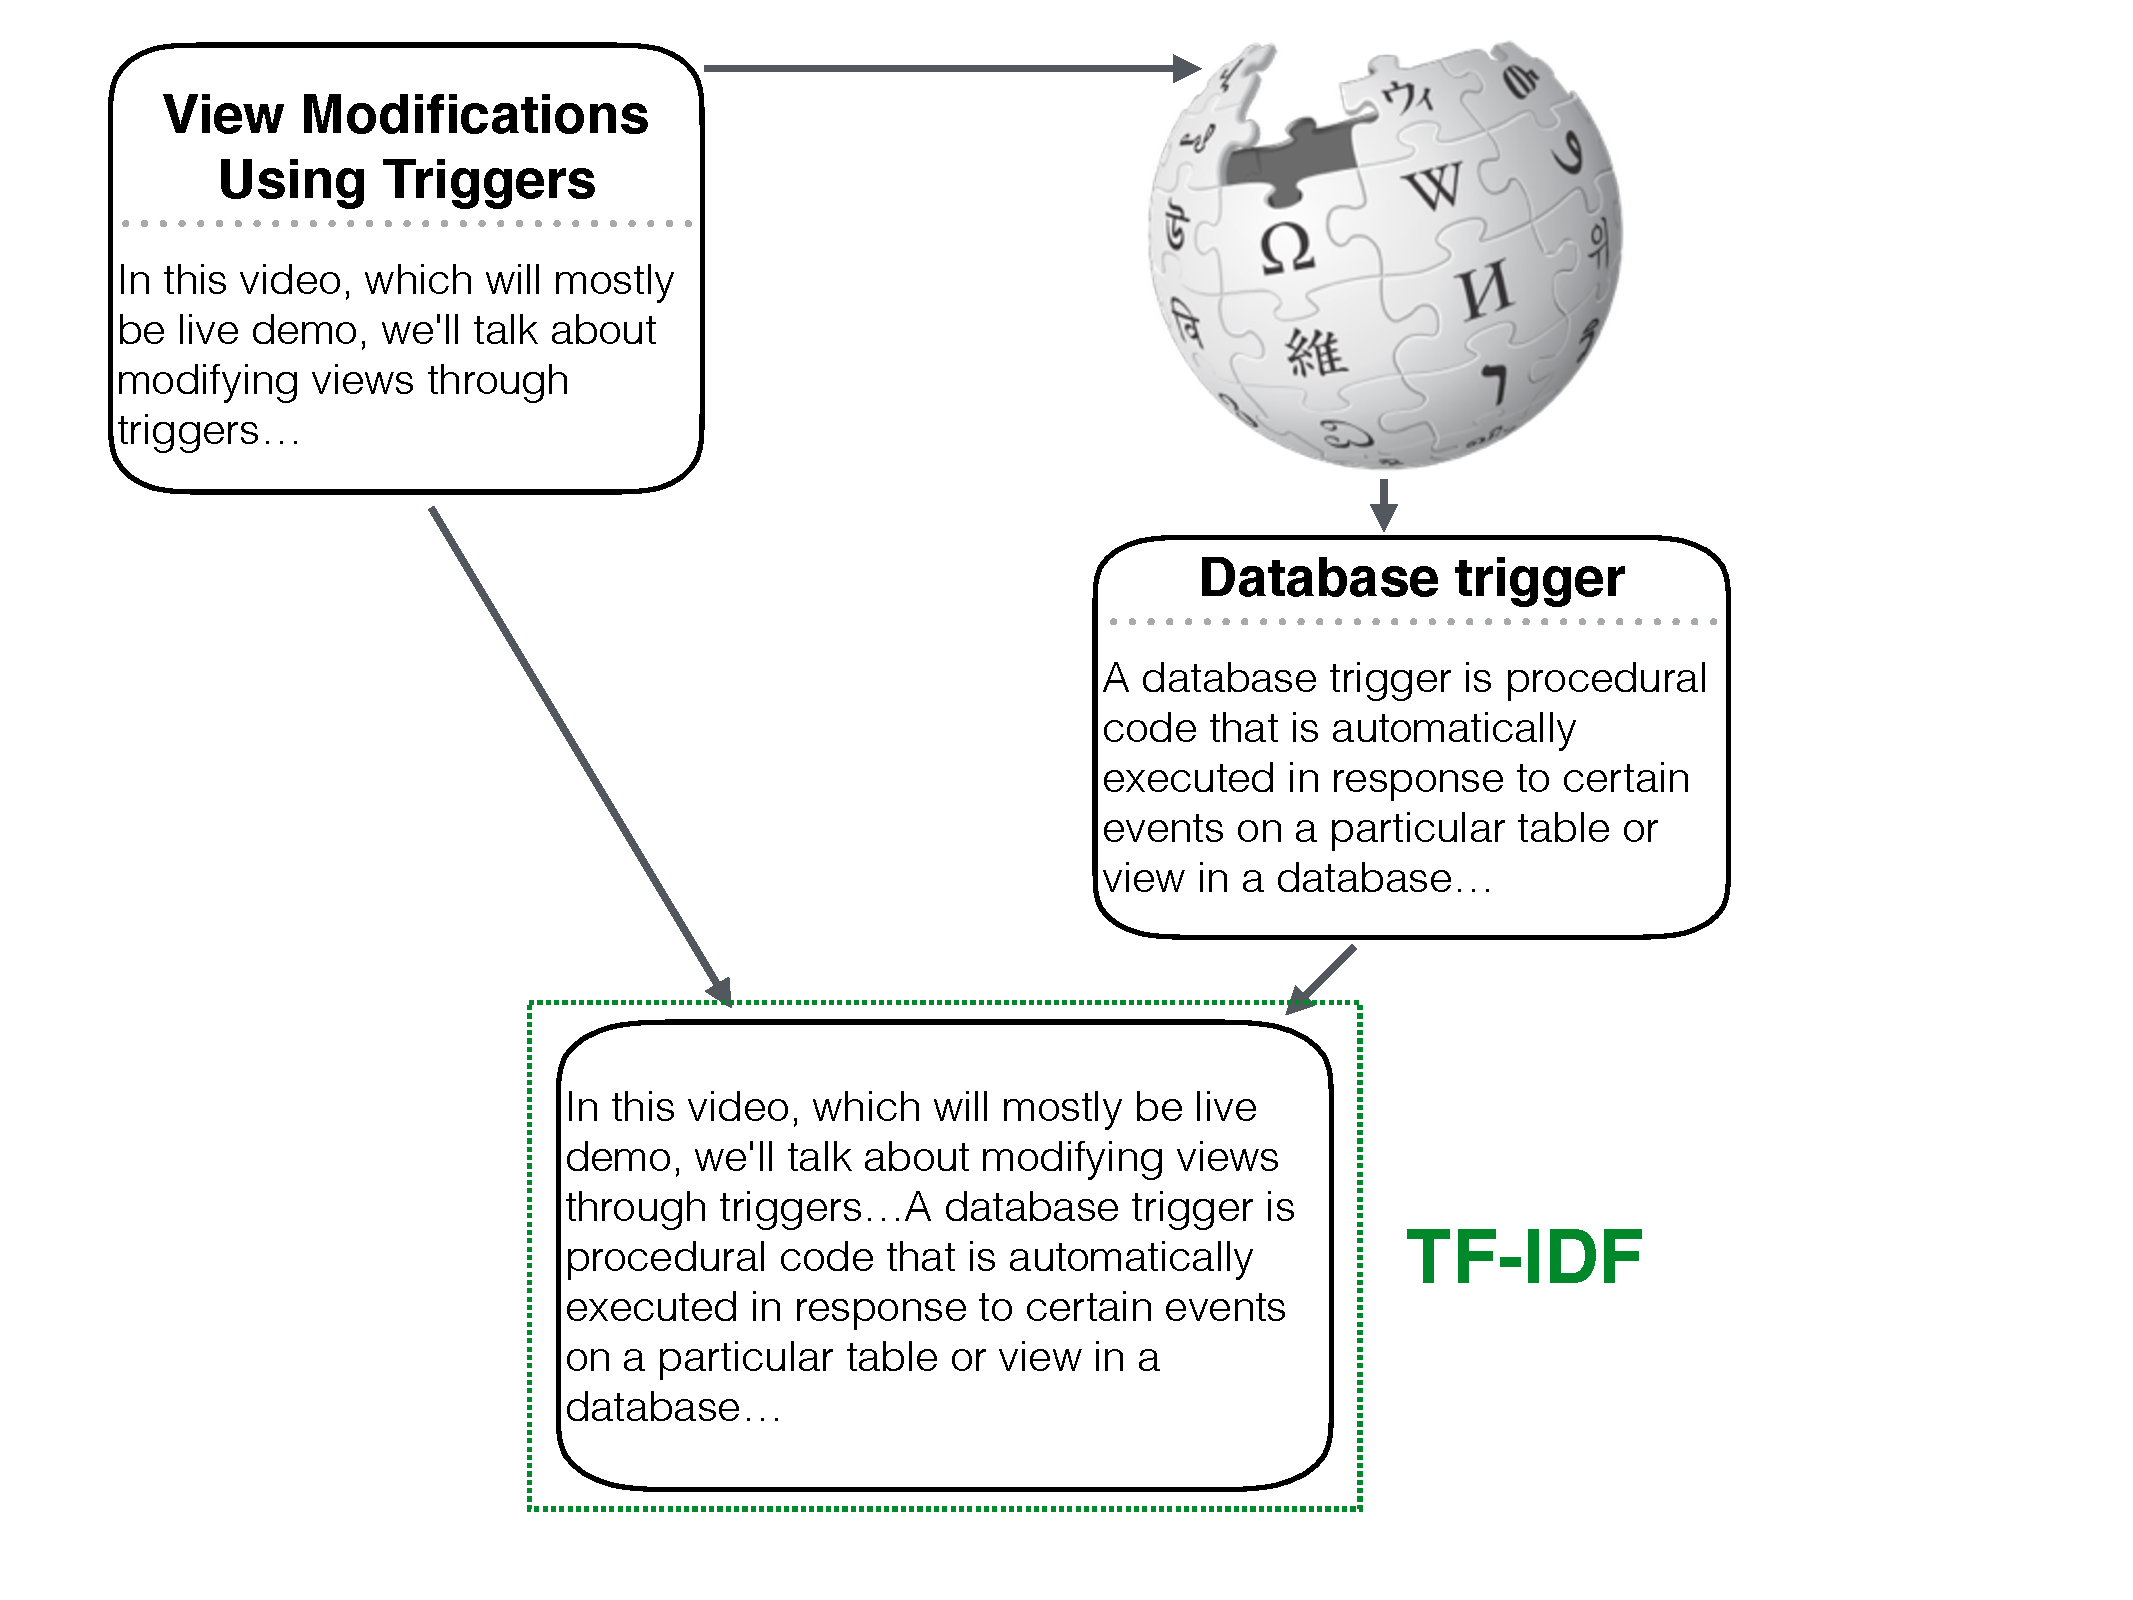
\includegraphics[width=\textwidth]{document_boosting.pdf}
\end{figure}

\subsubsection{Boosting Phrases}

This algorithm first creates a list of candidate index terms using
adjective-noun phrases. Then the candidates are ranked by their TF-IDF score
summed over all Wikipedia documents.

Next, this global candidate ranking is combined with the basic TF-IDF approach
described in Section~\ref{sec:tfidf} to form a final score that combines global
knowledge (from Wikipedia) with local knowledge (from the specific lecture video). 
%
% First, we create a normalized Wikipedia candidate ranking
% \begin{equation*}
% TF\text{-}IDF_{w-norm}(p, W) \coloneqq \frac{TF\text{-}IDF_w(p, W)}{\sum_{p'} TF\text{-}IDF_w(p', W)}
% \end{equation*}
% and normalized lecture collection ranking
% \begin{equation*}
% TF\text{-}IDF_{norm}(p, l, L) \coloneqq \frac{TF\text{-}IDF(p, l, L)}{\sum_{p'} TF\text{-}IDF(p', l, L)}
% \end{equation*}
% Then, we combine the two normalized rankings to form a final score
% \begin{multline*}
% TF\text{-}IDF_{combined}(p, l, L, W) \coloneqq \\ \eta TF\text{-}IDF_{w-norm}(p, W) + TF\text{-}IDF_{norm}(p, l, L)
% \end{multline*}
% where $\eta$ is used to determine the weight between Wikipedia scores
% and lecture scores.

We also experimented with only boosting phrases of at least two words,
based on the intution that longer phrases are often meaningful, but
appear infrequently and are therefore given low scores by TF-IDF. We
call this alternative ``Phrase Boosting N-Grams'' in Figure
\ref{fig:main_result}.
%
% A few subtleties deserve further description. First, in our simple
% TF-IDF approach, a score is calculated for each lecture $l$ and phrase
% $p$, while in our Wikipedia calculation a score is only calculated for
% each $p$. That approach is chosen because in this algorithm we are not interested in
% keywords for every Wikipedia document, but only in obtaining a global sense
% of the importance of a phrase. The algorithm is equivalent to summing over all
% Wikipedia documents $d \in W$
% \begin{equation*}
% TF_w(p) = \log \left(\sum_{d \in W} \text{number of times } p \text{ appears in } d\right)
% \end{equation*}
%
% Second, we take the logarithm of the phrase count in the Wikipedia
% ranking. This choice produces improved empirical results.
%
% \begin{figure}
% \caption{The Phrase Boosting algorithm runs TF-IDF over the entirety of Wikipedia and then combines the global ranking with a local ranking for a document.}
% 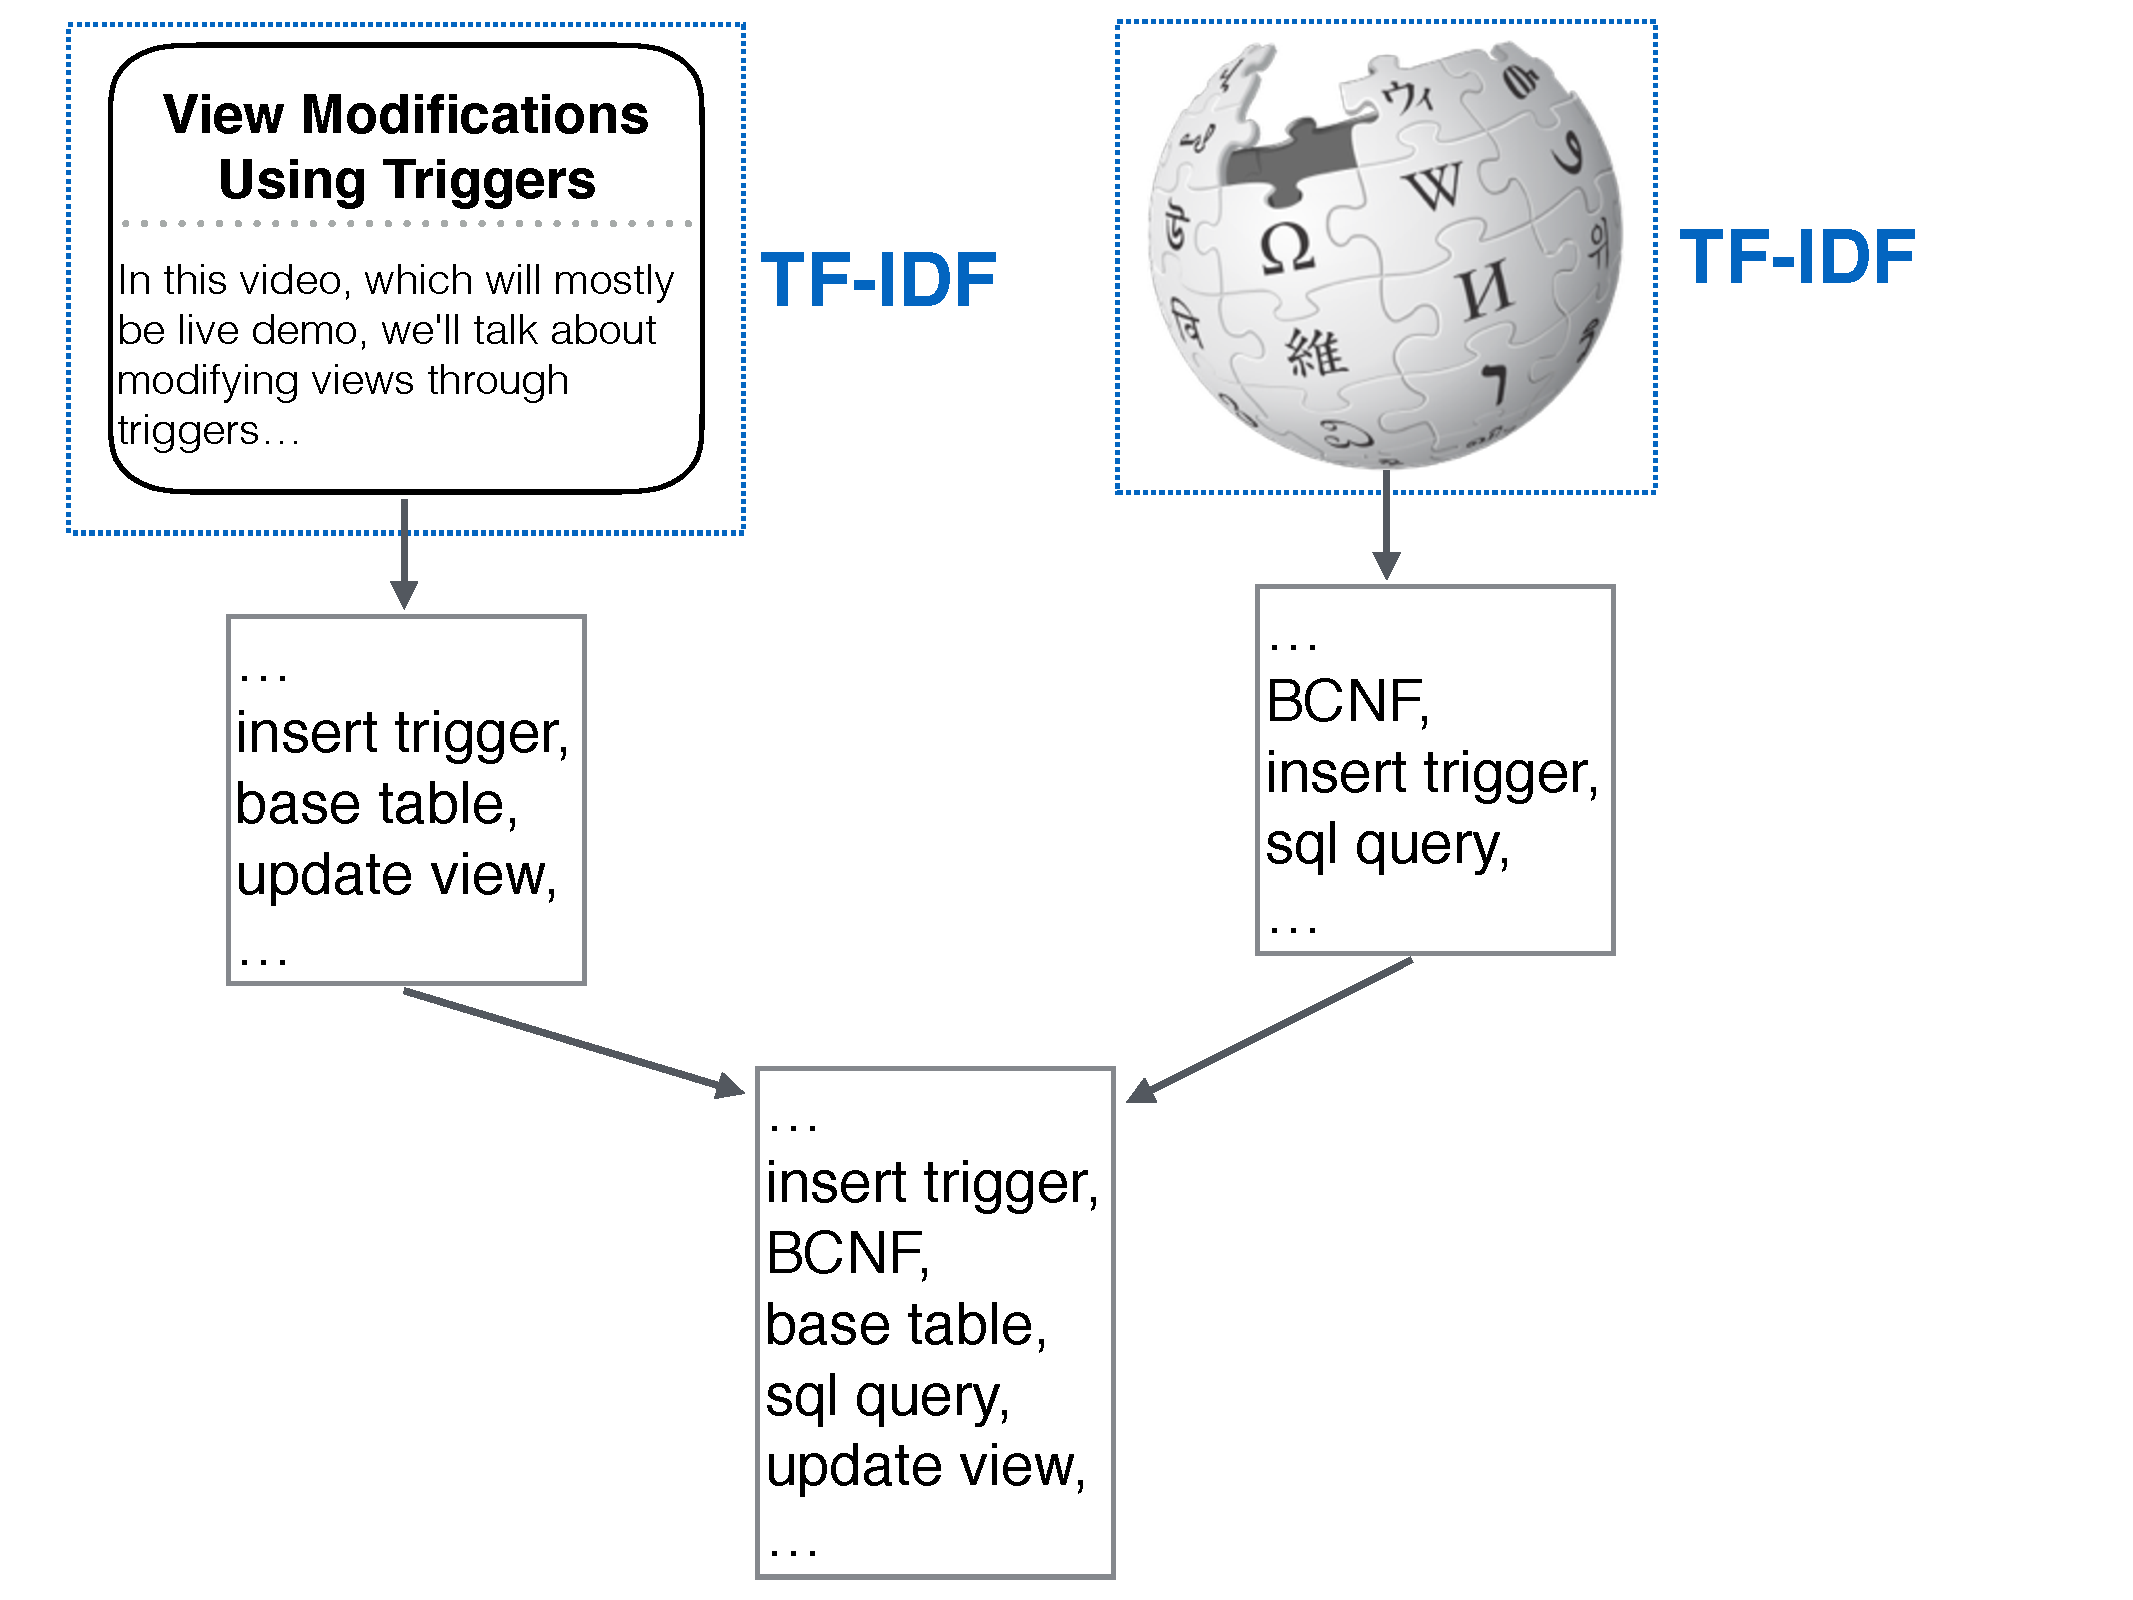
\includegraphics[width=\textwidth]{phrase_boosting.pdf}
% \end{figure}
